\newpage
\section{Materiais e métodos}
\label{sc:materias_e_metodos}

\subsection{Materiais}
\label{sc:materiais}

O sistema gerenciador de banco de dados alvo será o \textbf{PostgreSQL}~\cite{postgresql}, escolhido por ser de código aberto e amplamente utilizado. Para manter o escopo bem definido, dá-se suporte a um único banco, ficando a extensão a outros bancos relacionais como trabalho futuro. O ambiente de execução será o \textbf{Bun}~\cite{bun}, concorrente relevante ao Node.js na atualidade e em franco crescimento, cujo \emph{driver} \texttt{SQL} nativo~\cite{bun-sql} mediará todo o acesso ao banco.

\subsection{Métodos}
\label{sc:metodos}

A proposta combina uma escolha arquitetural --- o padrão \emph{Data Mapper} --- com a metaprogramação como método central, aplicada ao mapeamento objeto-relacional em duas frentes complementares: \emph{decorators} no momento da definição das classes e programação em nível de tipos no momento da compilação.

\textbf{Padrão de persistência.} Adota-se o padrão \emph{Repository}~\cite[p.~309]{fowler} por entidade, que faz mediação entre o domínio e a camada de mapeamento com uma interface semelhante a uma coleção, sobre a qual se consulta sem escrever SQL. Isolar a persistência em uma camada explícita mantém visível cada acesso ao banco, atacando o problema do N+1 apresentado na revisão: o acesso deixa de ocorrer implicitamente ao percorrer objetos.

\textbf{Composição de consultas.} As leituras sobre cada repositório são expressas por um \emph{query builder}, no sentido apresentado na revisão (Seção~\ref{sc:revisao}): a consulta é montada por encadeamento de operações, sem SQL em texto, e verificada pelo sistema de tipos em compilação, antes de ser traduzida para SQL parametrizado.

\textbf{Mapeamento por decorators.} Cada entidade é modelada como uma classe TypeScript cujos \emph{decorators} declaram o mapeamento objeto-relacional na própria definição da classe: que campos são colunas, qual é a chave primária e quais são as relações. Essa declaração é registrada quando a classe é definida e consumida pelo ORM em tempo de execução; a própria classe é a fonte da verdade do esquema. A título de ilustração, o trecho a seguir declara duas entidades, \texttt{User} e \texttt{Profile}, e a relação entre elas.

\begin{lstlisting}[language=Java,escapechar=|,caption={Declaração de entidades com os \emph{decorators} do OOR.},label={lst:decorators}]
@Entity(database)
class User {
  @PrimaryColumn({
    type: COLUMN_TYPE.TEXT,
    autogeneration: { clientSide: () => randomUUID() },
  })
  id?: PrimaryKey<string>;

  @Column({ type: COLUMN_TYPE.TEXT })
  @NotNullable
  name!: string;

  @ToOne({ target: () => Profile })
  @Nullable
  profile?: Profile;
}

@Entity(database)
class Profile {
  @PrimaryColumn({
    type: COLUMN_TYPE.SERIAL,
    autogeneration: { dbSide: () => undefined },
  })
  id?: PrimaryKey<number>;

  @Column({ type: COLUMN_TYPE.TEXT })
  @NotNullable
  bio!: string;
}

@Entity(database)
class Admin extends User {
  @Column({ type: COLUMN_TYPE.TEXT })
  @NotNullable
  department!: string;
}
\end{lstlisting}

Cada classe recebe \texttt{@Entity}, que a registra como entidade mapeada de um banco específico, passado como argumento. Dentro dela, \texttt{@PrimaryColumn} declara a chave primária, com seu tipo de coluna e a forma de geração do valor: em \texttt{User}, do lado da aplicação, por um identificador produzido antes da inserção (\texttt{clientSide}); em \texttt{Profile}, do lado do banco, por uma coluna \texttt{SERIAL} que o próprio PostgreSQL preenche (\texttt{dbSide}). \texttt{@Column} marca um campo como coluna comum e \texttt{@NotNullable} lhe impõe a restrição \texttt{NOT NULL}. 

As relações são declaradas no mesmo lugar: \texttt{@ToOne} estabelece uma relação para-um com outra entidade, indicada por uma função que devolve a classe-alvo (\texttt{() => Profile}); \texttt{@Nullable} torna a relação opcional. Por fim, a anotação de tipo do campo (\texttt{PrimaryKey<...>}) e os modificadores \texttt{?} e \texttt{!} indicam, no nível de tipos, o que é chave, opcional ou obrigatório.

O esquema relacional que essa declaração gera está representado na Figura~\ref{fig:modelo-fisico}: cada entidade torna-se uma tabela, cada \texttt{@Column} uma coluna e a relação \texttt{@ToOne} uma coluna de chave estrangeira (\texttt{profile\_id}) em \texttt{users}, que referência a chave primária de \texttt{profile}.

\begin{figure}[ht]
  \centering
  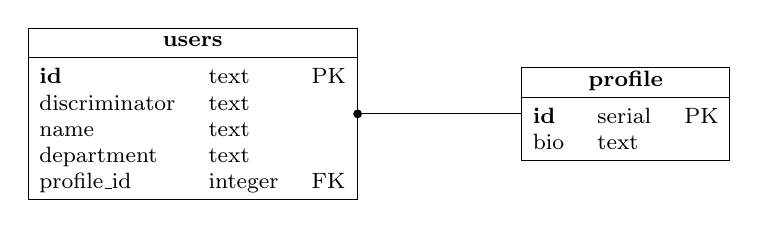
\begin{tikzpicture}[
    entity/.style={draw, inner sep=0pt},
    font=\footnotesize,
  ]
    \node[entity] (users) at (0,0) {%
      \begin{tabular}{@{\hspace{4pt}}l l l@{\hspace{4pt}}}
        \multicolumn{3}{@{}c@{}}{\textbf{users}} \\[1pt] \hline \\[-7pt]
        \textbf{id}   & text    & PK \\
        discriminator & text    &    \\
        name          & text    &    \\
        department    & text    &    \\
        profile\_id   & integer & FK \\[1pt]
      \end{tabular}%
    };
    \node[entity] (profile) at (5.5,0) {%
      \begin{tabular}{@{\hspace{4pt}}l l l@{\hspace{4pt}}}
        \multicolumn{3}{@{}c@{}}{\textbf{profile}} \\[1pt] \hline \\[-7pt]
        \textbf{id} & serial & PK \\
        bio         & text   &    \\[1pt]
      \end{tabular}%
    };
    \draw (users.east) -- (profile.west);
    \fill (users.east) circle (1.6pt);
  \end{tikzpicture}
  \caption{Modelo físico do banco gerado pelo exemplo da Listagem~\ref{lst:decorators}, com \texttt{User} e \texttt{Admin} acomodados na tabela \texttt{users} pela estratégia de tabela única.}
  \label{fig:modelo-fisico}
\end{figure}

\textbf{Herança de entidades (STI).} No exemplo, \texttt{Admin} estende \texttt{User} e acrescenta a coluna \texttt{department}, sem qualquer \emph{decorator} de configuração de herança. A herança entre entidades é reconhecida automaticamente ao se persistir duas ou mais classes de uma mesma hierarquia, e o ORM a realiza pela estratégia de tabela única apresentada na revisão, acomodando \texttt{User} e \texttt{Admin} na mesma tabela \texttt{users} e escrevendo na coluna discriminadora \texttt{discriminator} o subtipo de cada linha. As colunas próprias do subtipo, como \texttt{department}, admitem valor nulo nas linhas dos demais tipos. Preserva-se assim, no banco, a herança que o código expressa, sem que o domínio conheça a forma de armazenamento.

\textbf{Programação em nível de tipos (compilação).} A segunda frente emprega o sistema de tipos para levar a verificação de correção do mapeamento do tempo de execução para o tempo de compilação: a partir da declaração de cada entidade, as operações de persistência são tipadas de modo que usos inválidos --- omitir dados obrigatórios ou referir-se a campos inexistentes --- sejam rejeitados pelo compilador, antes da execução.

